\chapter{Analisi di centralità}
\label{cap4}
Dopo aver descritto le principali caratteristiche strutturali e topologiche della rete metropolitana milanese, è possibile approfondire lo studio del grafo analizzandone le misure di \textbf{centralità}. \\
Queste metriche consentono di valutare l’importanza relativa dei nodi all’interno della rete, non solo in termini di numero di connessioni, ma anche di posizione strategica e di ruolo funzionale nella connettività complessiva del sistema.

\section{Centralità di grado}
La \textbf{degree centrality} indica quanti collegamente diretti o \textit{adiacenze} ha ciascun nodo della rete. Nella figura \ref{fig: Degree Centrality} è rappresentata la distribuzione di questa misurazione.

\vspace{1em}
\begin{figure}[h!]
    \centering
    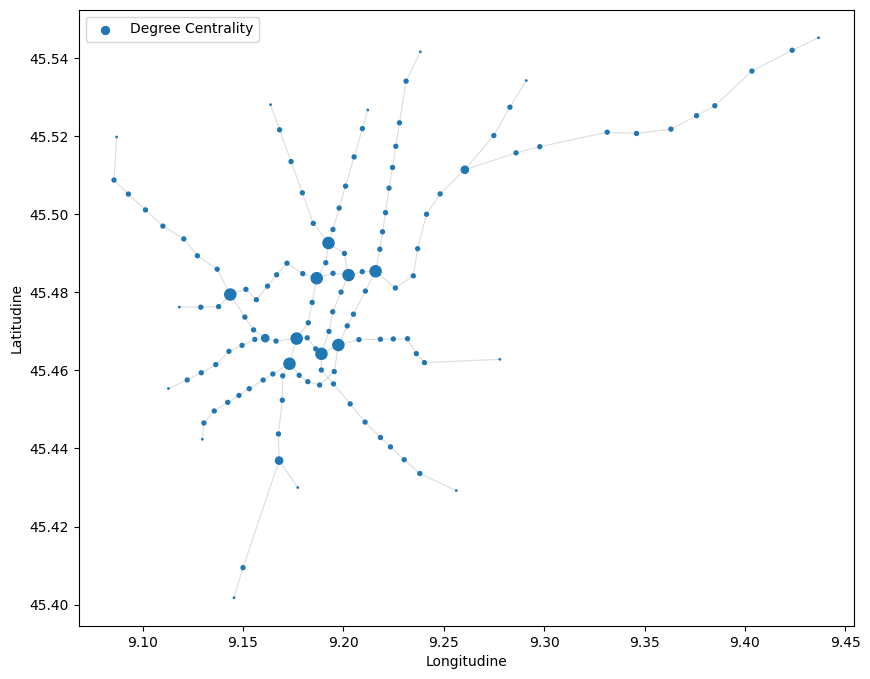
\includegraphics[width=0.8\linewidth]{Immagini//Capitoli//cap4/degree_centr.png}
    \caption{Degree centrality}
    \label{fig: Degree Centrality}
\end{figure}
\vspace{1em}

Valgono tutte le considerazioni sui gradi già affrontante nel corso del capitolo \ref{cap3}.


\section{Centralità di intermediazione}
La \textbf{betweeness centrality} misura quante volte un nodo si trova in un \textit{percorso minimo} tra altre coppie di nodi, ovvero identifica i nodi più rilevanti come quelli che fanno da ponte tra due gruppi di nodi.

\vspace{1em}
\begin{figure}[h!]
    \centering
    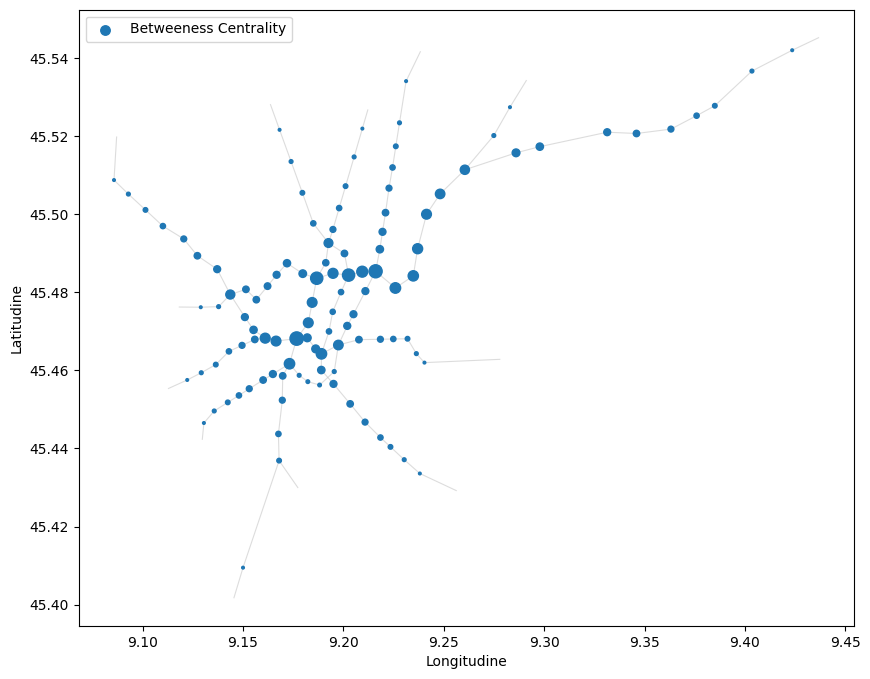
\includegraphics[width=0.8\linewidth]{Immagini//Capitoli//cap4/betw_centr.png}
    \caption{Betweeness centrality}
    \label{fig: Betweeness Centrality}
\end{figure}
\vspace{1em}

In figura \ref{fig: Betweeness Centrality} è rappresentata la distribuzione di questa misurazione, si osserva che i nodi centrali e quelli precedenti a delle diramazioni hanno un'importanza maggiore rispetto ai nodi presenti su diramazioni periferiche.

\subsection{Nodi centrali di intermediazione}
Come ci si potrebbe aspettare, i nodi centrali secondo questa misurazione sono \textit{principalmente} quelli di interscambio, ma ci sono comunque alcuni nodi che, nonostante non siano di interscambio, hanno un alto potere di intermediazione, infatti verificando i primi dieci nodi per centralità di intermediazione:

\begin{center}
CADORNA \\
LORETO \\
GARIBALDI FS \\
CENTRALE FS \\
CAIAZZO \\
PIOLA \\
DUOMO \\
SAN AMBROGIO \\
LAMBRATE FS \\
UDINE \\
\end{center}

si ritrova \textit{ad esempio} la stazione di \textit{PIOLA} prima di quella di \textit{DUOMO}, come alcune stazioni \textit{non} geograficamente centrali come \textit{LAMBRATE FS} e \textit{UDINE}.

\section{Centralità di prossimità}
La \textbf{closeness centality} misura quanto un nodo è vicino, in termini di distanza nel grafo, da tutti gli altri nodi.

\vspace{1em}
\begin{figure}[h!]
    \centering
    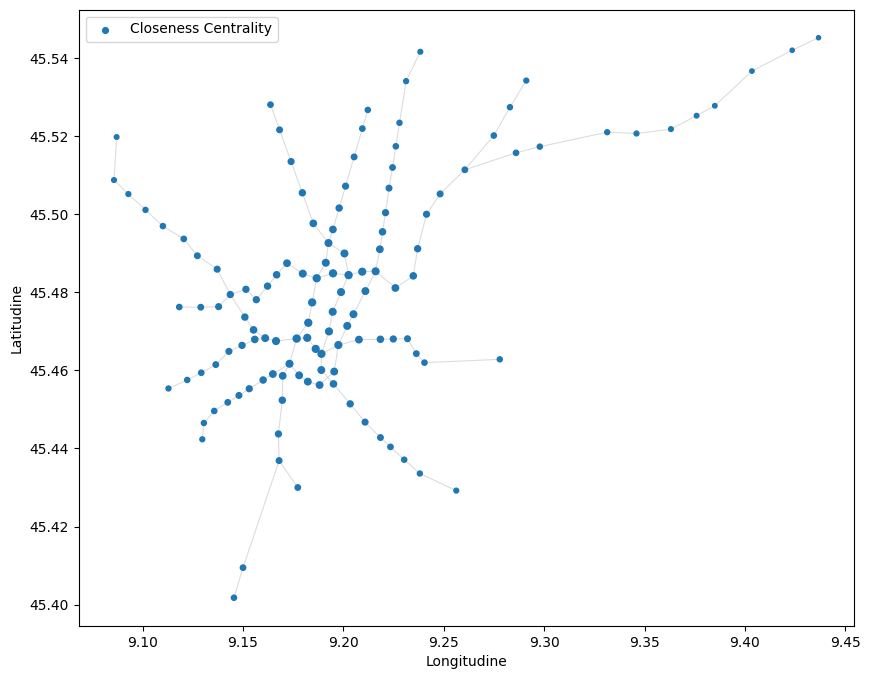
\includegraphics[width=0.8\linewidth]{Immagini//Capitoli//cap4/close_centr.png}
    \caption{Closeness centrality}
    \label{fig: Closeness Centrality}
\end{figure}
\vspace{1em}

In figura \ref{fig: Closeness Centrality} è rappresentata la distribuzione di questa misurazione.

\subsection{Nodi centrali di prossimità}
Anche in questo caso, i nodi più centrali sono quelli che sono anche \textit{geograficamente} più centrali. Più interessante per questa misurazione è invece capire quali nodi sono meno centrali, che intuitivamente dovrebbero essere quelli agli estremi delle diramazioni più lontane dal centro, ovvero la diramazione per \textit{RHO FIERAMILANO} della linea 1 e la diramazione per \textit{GESSATE} della linea 2. In effetti, gli ultimi 8 nodi per centralità di prossimità sono:

\begin{center}
GESSATE \\
CASCINA ANTONIETTA \\
GORGONZOLA \\
VILLA POMPEA \\
BUSSERO \\
RHO FIERAMILANO \\
CASSINA DE PECCHI \\
PERO \\
\end{center}

che sono, a conferma di quanto ipotizzato, proprio stazioni appartenenti alle diramazioni precedentemente evidenziate.

\section{Centralità di autovettore}
La \textbf{eigenvector centrality} valuta l'importanza di un nodo in funzione dell'importanza dei suoi vicini, ovvero un nodo è importante se collegato ad altri nodi importanti.

\vspace{1em}
\begin{figure}[h!]
    \centering
    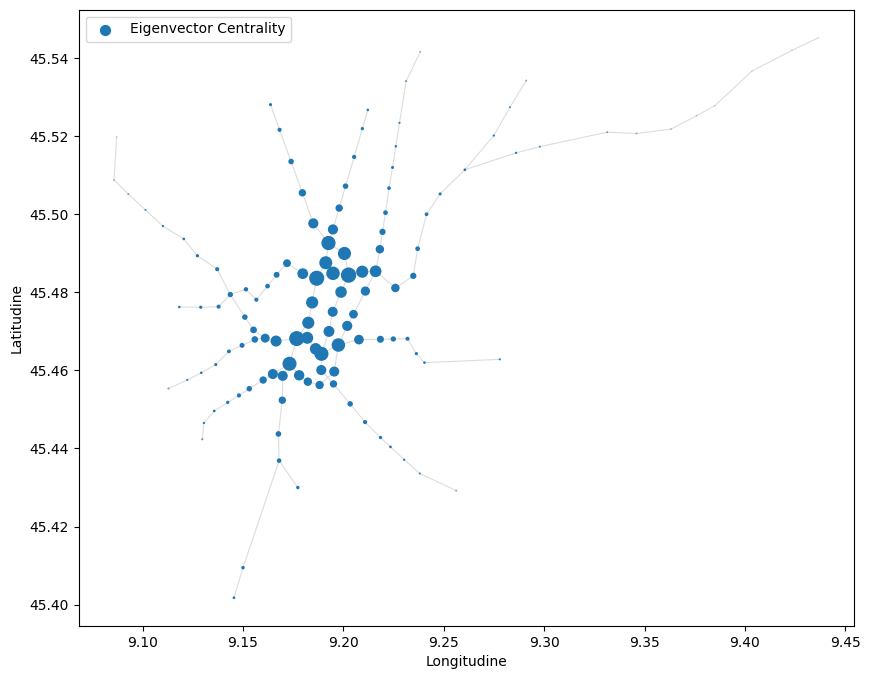
\includegraphics[width=0.8\linewidth]{Immagini//Capitoli//cap4/eigen_centr.png}
    \caption{Eigenvector centrality}
    \label{fig: Eigenvector Centrality}
\end{figure}
\vspace{1em}

In figura \ref{fig: Eigenvector Centrality} è rappresentata la distribuzione di questa misurazione, in cui è maggiormente evidente, rispetto alle altre misure di centralità, quanto i nodi corrispondenti a stazioni \textit{geograficamente} più centrali siamo più importanti rispetto ai nodi periferici, che in questa misurazione diventano del tutto trascurabili e anche difficilmente leggibili in figura.